\begin{frame}
\frametitle{NLG System Architecture}

Reiter and Dale suggest a three-stage pipeline:

\vspace{12pt}

\begin{center}
% Illustration of three-stage NLG system architecture
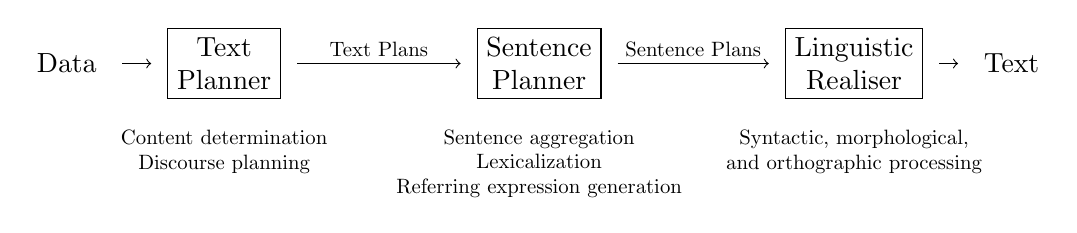
\begin{tikzpicture}

\node(0) [align=center, outer sep=6pt] at (-2, 0) {Data};

\node(1) [rectangle, draw, align=center, outer sep=6pt] at (0, 0) {Text \\ Planner};
\node [align=center, scale=0.75, below of=1, anchor=north] {
	Content determination\\
	Discourse planning
};

\node(2) [rectangle, draw, align=center, outer sep=6pt] at (4, 0) {Sentence \\ Planner};
\node [align=center, scale=0.75, below of=2, anchor=north] {
	Sentence aggregation\\
	Lexicalization\\
	Referring expression generation
};

\node(3) [rectangle, draw, align=center, outer sep=6pt] at (8, 0) {Linguistic \\ Realiser};
\node [align=center, scale=0.75, below of=3, anchor=north] {
	Syntactic, morphological,\\
	and orthographic processing
};

\node(4) [align=center, outer sep=6pt] at (10, 0) {Text};

\draw [->] (0) -- (1);
\draw [->] (1) to node[above, scale=0.75] {Text Plans} (2);
\draw [->] (2) to node[above, scale=0.75] {Sentence Plans} (3);
\draw [->] (3) -- (4);

\end{tikzpicture}

\end{center}

\vspace{12pt}

We need two more data objects to represent the data passed between
stages in the pipeline:

\begin{itemize}
	\item \textbf{Text plans} specify messages and how they are conceptually grouped
	\item \textbf{Sentence plans} specify templates or abstract representations of sentences
\end{itemize}
\end{frame}
